\section{Cảm biến \& Computational Imaging: Vượt ra ngoài Giới hạn Truyền thống}
\label{sec:advanced_sensors_computational_imaging}

\subsection{Giới thiệu: Mở rộng Khả năng Tri giác của Máy móc}
\label{subsec:advanced_sensors_intro}

Trong nhiều thập kỷ, mô hình camera truyền thống—với cảm biến khung hình (frame-based) và dải động giới hạn—đã là "đôi mắt" mặc định cho các hệ thống Thị giác Máy tính. Mô hình này, mặc dù thành công, về cơ bản là một sự mô phỏng đơn giản hóa của cách thế giới thị giác được ghi lại. Nó hoạt động theo một nhịp đồng hồ toàn cục, chụp lại toàn bộ cảnh tại những khoảnh khắc rời rạc, bất kể cảnh đó đang tĩnh lặng hay chuyển động dữ dội. Nó cũng bị giới hạn bởi một dải cường độ sáng hẹp, thường dẫn đến tình trạng cháy sáng hoặc tối đen trong các cảnh có độ tương phản cao.

Tuy nhiên, thiên nhiên và kỹ thuật đã chỉ ra những con đường khác. Hệ thống thị giác sinh học không hoạt động theo từng khung hình; nó phản ứng với sự thay đổi một cách bất đồng bộ. Thế giới thực cũng không bị giới hạn trong dải động hẹp. Sự ra đời của các loại cảm biến mới và các kỹ thuật \textbf{Computational Imaging} (Nhiếp ảnh Tính toán) đang mở ra một kỷ nguyên mới cho Thị giác Máy tính, nơi chúng ta có thể thu nhận thông tin thị giác một cách phong phú và hiệu quả hơn bao giờ hết, vượt qua những giới hạn cố hữu của camera truyền thống.

Computational Imaging là một lĩnh vực liên ngành kết hợp thiết kế quang học, cảm biến, và các thuật toán xử lý tín hiệu để cùng nhau giải quyết một bài toán. Thay vì chỉ dựa vào phần cứng quang học để tạo ra một bức ảnh hoàn chỉnh, nó thu nhận một dạng dữ liệu "mã hóa" và sau đó sử dụng sức mạnh tính toán để "giải mã" và tái tạo lại một phiên bản tốt hơn hoặc một dạng thông tin hoàn toàn mới.

Trong phần này, chúng ta sẽ khám phá ba trong số những đổi mới đột phá nhất trong lĩnh vực này:
\begin{itemize}
    \item \textbf{Event-based Vision (Thị giác dựa trên Sự kiện):} Một mô hình cảm biến lấy cảm hứng từ sinh học, hoạt động bất đồng bộ và chỉ ghi lại sự thay đổi, mở ra tiềm năng cho các ứng dụng tốc độ cực cao và năng lượng cực thấp.
    \item \textbf{High Dynamic Range (HDR) Imaging (Ảnh dải Động Rộng):} Các kỹ thuật cho phép camera "nhìn thấy" chi tiết trong cả vùng sáng nhất và tối nhất của một cảnh, giống như mắt người.
    \item \textbf{Light Field (Plenoptic) Imaging (Ảnh Trường sáng):} Một phương pháp thu nhận không chỉ cường độ và màu sắc của ánh sáng, mà còn cả hướng của các tia sáng, cho phép các khả năng hậu kỳ kỳ diệu như lấy nét lại sau khi chụp và tạo ra các góc nhìn khác nhau từ một lần chụp duy nhất.
\end{itemize}

Việc tìm hiểu các công nghệ này không chỉ là một sự cập nhật về phần cứng, mà còn là một sự thay đổi về tư duy: làm thế nào chúng ta có thể thiết kế các hệ thống thị giác toàn diện, nơi cảm biến và thuật toán cùng nhau hợp tác để thu nhận thông tin một cách thông minh hơn.

\subsection{Event-based Vision: Cuộc cách mạng Bất đồng bộ}
\label{subsec:event_based_vision}

\subsubsection{Hạn chế của Cảm biến Khung hình Truyền thống}
\label{subsubsec:frame_based_limitations}
Cảm biến CMOS/CCD truyền thống hoạt động giống như một chiếc máy photocopy tốc độ cao. Tại những khoảng thời gian cố định (được quyết định bởi \textit{tốc độ khung hình - frame rate}), nó "đóng băng" toàn bộ cảnh và ghi lại giá trị cường độ sáng tại mỗi pixel. Mô hình này có ba hạn chế cố hữu:
\begin{enumerate}
    \item \textbf{Độ trễ (Latency):} Toàn bộ khung hình phải được phơi sáng, sau đó được đọc ra tuần tự từ cảm biến. Quá trình này tạo ra một độ trễ cố hữu, thường là hàng chục mili giây. Đối với các ứng dụng tốc độ cao như theo dõi robot hay điều hướng drone, độ trễ này là quá lớn.
    \item \textbf{Sự dư thừa Dữ liệu (Data Redundancy):} Trong một cảnh tĩnh hoặc gần tĩnh (ví dụ: một cuộc họp video), phần lớn các pixel không thay đổi giữa các khung hình. Tuy nhiên, camera truyền thống vẫn ghi lại và truyền đi toàn bộ dữ liệu của tất cả các pixel, gây lãng phí băng thông và năng lượng tính toán.
    \item \textbf{Nhòe Chuyển động (Motion Blur):} Khi một vật thể di chuyển nhanh trong thời gian phơi sáng, ánh sáng từ vật thể đó sẽ trải dài trên nhiều vị trí của pixel, tạo ra hiện tượng nhòe. Điều này làm mất đi các chi tiết quan trọng.
    \item \textbf{Dải Động (Dynamic Range) Hạn chế:} Tất cả các pixel trên cùng một cảm biến phải chia sẻ chung một thời gian phơi sáng. Điều này khiến camera khó có thể xử lý các cảnh có độ tương phản cao, dẫn đến cháy sáng ở vùng sáng và mất chi tiết ở vùng tối.
\end{enumerate}

\subsubsection{Nguyên lý hoạt động của Cảm biến Sự kiện}
\label{subsubsec:event_camera_principles}
Lấy cảm hứng từ hệ thống thị giác sinh học, \textbf{cảm biến sự kiện (event camera)}, hay còn gọi là Dynamic Vision Sensor (DVS), hoạt động theo một nguyên lý hoàn toàn khác: \textbf{bất đồng bộ và dựa trên sự thay đổi} \cite{Gallego2020}.

Thay vì một bộ đếm thời gian toàn cục, mỗi pixel trên cảm biến sự kiện hoạt động độc lập và có mạch xử lý riêng. Mỗi pixel liên tục theo dõi cường độ sáng logarit của ánh sáng chiếu vào nó. Nó chỉ tạo ra một "sự kiện" (event) khi sự thay đổi của cường độ sáng logarit này vượt qua một ngưỡng nhất định, $C$.
\begin{equation}
    \log(I(t)) - \log(I(t_{\text{last}})) \ge \pm C
\end{equation}
Một sự kiện là một gói dữ liệu nhỏ gọn chứa:
\begin{itemize}
    \item \textbf{Tọa độ (x, y):} Vị trí của pixel đã kích hoạt.
    \item \textbf{Dấu thời gian (timestamp, t):} Thời điểm chính xác xảy ra sự kiện, với độ phân giải micro giây.
    \item \textbf{Cực tính (polarity, p):} Hướng của sự thay đổi (+1 cho tăng sáng, -1 cho giảm sáng).
\end{itemize}
\begin{equation}
    \text{event} = (x, y, t, p)
\end{equation}
Kết quả đầu ra của cảm biến không phải là một chuỗi các hình ảnh, mà là một dòng chảy liên tục, thưa thớt của các sự kiện này.

\begin{center}
    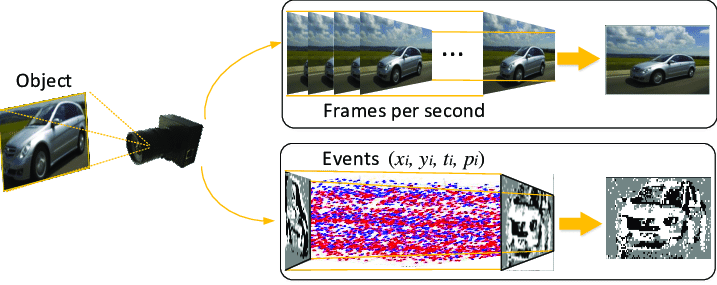
\includegraphics[width=1.0\textwidth]{images/event_camera_principle.png}
    \captionof{figure}{So sánh giữa camera truyền thống và camera sự kiện. (Trên) Camera truyền thống ghi lại các khung hình đầy đủ tại các khoảng thời gian cố định. (Dưới) Camera sự kiện hoạt động bất đồng bộ, chỉ tạo ra một sự kiện tại pixel khi có sự thay đổi đủ lớn về độ sáng, tạo ra một dòng dữ liệu không-thời gian thưa thớt.}
    \label{fig:event_camera_principle}
\end{center}

\subsubsection{Ưu điểm và Thách thức}
\label{subsubsec:event_camera_pros_cons}
Mô hình hoạt động này mang lại những ưu điểm vượt trội:
\begin{description}
    \item[Độ phân giải Thời gian Cực cao:] Vì các sự kiện được ghi lại với dấu thời gian micro giây, camera có thể theo dõi các chuyển động cực nhanh mà không bị nhòe.
    \item[Dải Động Rộng (High Dynamic Range - HDR):] Mỗi pixel tự điều chỉnh độ nhạy của nó một cách độc lập. Điều này cho phép cảm biến hoạt động tốt trong các cảnh có dải động lên tới 120-140 dB, có thể nhìn thấy chi tiết cả trong nhà và ngoài cửa sổ nắng gắt cùng một lúc.
    \item[Năng lượng Tiêu thụ Thấp và Dữ liệu Thưa thớt:] Trong một cảnh tĩnh, camera gần như không tạo ra sự kiện nào và tiêu thụ rất ít năng lượng. Dữ liệu chỉ được tạo ra khi có chuyển động, giúp giảm đáng kể yêu cầu về băng thông và xử lý.
\end{description}
Tuy nhiên, những ưu điểm này đi kèm với một thách thức lớn: \textbf{toàn bộ các thuật toán Thị giác Máy tính truyền thống được thiết kế cho các hình ảnh dạng lưới dày đặc không thể áp dụng trực tiếp}. Dữ liệu sự kiện là một đám mây điểm không-thời gian, thưa thớt và không có cấu trúc. Điều này đòi hỏi phải phát triển các phương pháp biểu diễn và xử lý hoàn toàn mới, chẳng hạn như:
\begin{itemize}
    \item \textbf{Tái tạo ảnh từ sự kiện:} Chuyển đổi dòng sự kiện thành các hình ảnh có thể xử lý bằng các mạng CNN truyền thống.
    \item \textbf{Xử lý trực tiếp trên dòng sự kiện:} Sử dụng các mạng nơ-ron đồ thị (Graph Neural Networks) hoặc các mạng nơ-ron xung (Spiking Neural Networks - SNNs) để xử lý dữ liệu một cách tự nhiên hơn.
\end{itemize}

\subsection{High Dynamic Range (HDR) Imaging}
\label{subsec:hdr_imaging}

\subsubsection{Vấn đề về Dải động}
\label{subsubsec:dynamic_range_problem}
\textbf{Dải động (Dynamic Range)} của một cảnh là tỷ lệ giữa cường độ sáng mạnh nhất và yếu nhất. Mắt người có dải động tĩnh (static) khoảng 100:1 nhưng dải động thích ứng (adaptive) lên tới 1,000,000:1 nhờ khả năng điều chỉnh của con ngươi và võng mạc. Trong khi đó, một cảm biến camera truyền thống chỉ có dải động khoảng 1000:1 (tương đương 60 dB).
Khi chụp một cảnh có dải động lớn hơn dải động của cảm biến (ví dụ: một căn phòng có cửa sổ nhìn ra ngoài trời nắng), bộ phơi sáng của máy ảnh phải đưa ra một lựa chọn:
\begin{itemize}
    \item \textbf{Phơi sáng ngắn:} Giữ lại chi tiết ở vùng sáng (bầu trời ngoài cửa sổ), nhưng vùng tối (bên trong phòng) sẽ trở nên gần như đen kịt.
    \item \textbf{Phơi sáng dài:} Ghi lại chi tiết ở vùng tối, nhưng vùng sáng sẽ bị \textbf{cháy (clamped/saturated)} thành màu trắng hoàn toàn, mất hết thông tin.
\end{itemize}

\subsubsection{Giải pháp: Kết hợp Đa phơi sáng}
\label{subsubsec:multi_exposure_fusion}
Kỹ thuật HDR cơ bản nhất \cite{Debevec1997} hoạt động bằng cách chụp một loạt các ảnh cùng một cảnh với các mức phơi sáng khác nhau (thường gọi là \textbf{bracketing}), sau đó kết hợp chúng lại.
\begin{enumerate}
    \item \textbf{Chụp ảnh:} Chụp ít nhất ba ảnh: một ảnh thiếu sáng (underexposed), một ảnh đúng sáng (normally exposed), và một ảnh thừa sáng (overexposed).
    \item \textbf{Xây dựng Hàm Phản hồi Camera (Camera Response Function - CRF):} CRF là một hàm phi tuyến mô tả mối quan hệ giữa bức xạ (irradiance) thực tế chiếu vào cảm biến và giá trị pixel kỹ thuật số mà nó tạo ra. Bằng cách phân tích các giá trị pixel của cùng một điểm trong cảnh qua các mức phơi sáng khác nhau, ta có thể ước lượng được CRF.
    \item \textbf{Tái tạo Bản đồ Bức xạ (Radiance Map):} Sử dụng CRF đã ước lượng, các giá trị pixel từ tất cả các ảnh được chuyển đổi ngược lại thành các giá trị bức xạ tuyến tính. Sau đó, một bản đồ bức xạ HDR 32-bit float được tạo ra bằng cách lấy trung bình có trọng số của các giá trị này, ưu tiên các pixel được phơi sáng tốt (không quá tối, không quá cháy) từ mỗi ảnh.
    \item \textbf{Ánh xạ Tông màu (Tone Mapping):} Bản đồ bức xạ HDR có dải động quá lớn để có thể hiển thị trên màn hình 8-bit thông thường (Low Dynamic Range - LDR). Tone mapping là quá trình nén dải động của ảnh HDR xuống dải động của màn hình LDR, trong khi vẫn cố gắng bảo toàn chi tiết và độ tương phản cục bộ. Đây là một bước nghệ thuật cũng như kỹ thuật, và có nhiều thuật toán tone mapping khác nhau để tạo ra các phong cách hình ảnh khác nhau.
\end{enumerate}

\begin{center}
    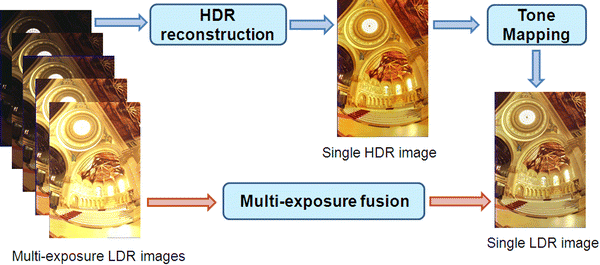
\includegraphics[width=1.0\textwidth]{images/hdr_pipeline.png}
    \captionof{figure}{Quy trình tạo ảnh HDR/LDR: chụp nhiều ảnh LDR, kết hợp thành HDR, ánh xạ tông màu sang LDR hoặc hợp nhất đa phơi sáng trực tiếp.}
    \label{fig:hdr_pipeline}
\end{center}

Các phương pháp dựa trên học sâu gần đây \cite{Wang2021Review} đang cố gắng thực hiện các bước này, hoặc thậm chí toàn bộ quy trình, bằng một mạng nơ-ron end-to-end, cho phép tái tạo HDR từ một ảnh LDR duy nhất hoặc căn chỉnh và kết hợp các ảnh đa phơi sáng một cách thông minh hơn.

\subsection{Light Field (Plenoptic) Imaging: Thu nhận cả Hướng tia sáng}
\label{subsec:light_field_imaging}

\subsubsection{Hàm Plenoptic và Trường sáng 4D}
\label{subsubsec:plenoptic_function}
Một hình ảnh truyền thống là một phép chiếu 2D của thế giới 3D. Nó trả lời câu hỏi: "Bao nhiêu ánh sáng đến từ mỗi hướng?". \textbf{Hàm Plenoptic} \cite{Adelson1991} là một khái niệm tổng quát hơn, mô tả toàn bộ thông tin thị giác có thể quan sát được từ mọi điểm trong không gian, theo mọi hướng, tại mọi thời điểm, và ở mọi bước sóng. Nó là một hàm 7 chiều: $P(x, y, z, \theta, \phi, \lambda, t)$.

\textbf{Trường sáng (Light Field)} là một phiên bản đơn giản hóa 4D của hàm Plenoptic, thường được ký hiệu là $L(u, v, s, t)$. Nó mô tả luồng ánh sáng đi qua một mặt phẳng trong không gian 3D.
\begin{itemize}
    \item $(u, v)$ là tọa độ của một tia sáng khi nó giao với một mặt phẳng (mặt phẳng cảm biến).
    \item $(s, t)$ là tọa độ của cùng tia sáng đó khi nó giao với một mặt phẳng thứ hai (mặt phẳng thấu kính).
\end{itemize}
\textbf{Trực giác:} Một hình ảnh truyền thống tích hợp (tổng hợp) tất cả các tia sáng đi qua mỗi điểm trên thấu kính và hội tụ tại một điểm trên cảm biến. Trường sáng không thực hiện bước tích hợp này; thay vào đó, nó ghi lại thông tin của từng tia sáng một cách riêng biệt.

\subsubsection{Cách hoạt động của Camera Trường sáng}
\label{subsubsec:light_field_camera_operation}
Một camera trường sáng, hay camera plenoptic, thực hiện điều này bằng cách đặt một \textbf{mảng vi thấu kính (microlens array)} giữa thấu kính chính và cảm biến hình ảnh \cite{Ng2005}.
\begin{itemize}
    \item Thấu kính chính hội tụ ánh sáng từ cảnh.
    \item Mảng vi thấu kính, nằm ngay trên cảm biến, hoạt động như một mảng các camera nhỏ. Mỗi vi thấu kính sẽ chụp một "hình ảnh nhỏ" của thấu kính chính từ góc nhìn của nó.
    \item Cảm biến ghi lại một mảng các hình ảnh nhỏ này.
\end{itemize}
Dữ liệu thô từ một camera trường sáng trông giống như một tấm ảnh tổ ong. Bằng cách phân tích dữ liệu này, chúng ta có thể tái cấu trúc lại trường sáng 4D $L(u, v, s, t)$.

\begin{center}
    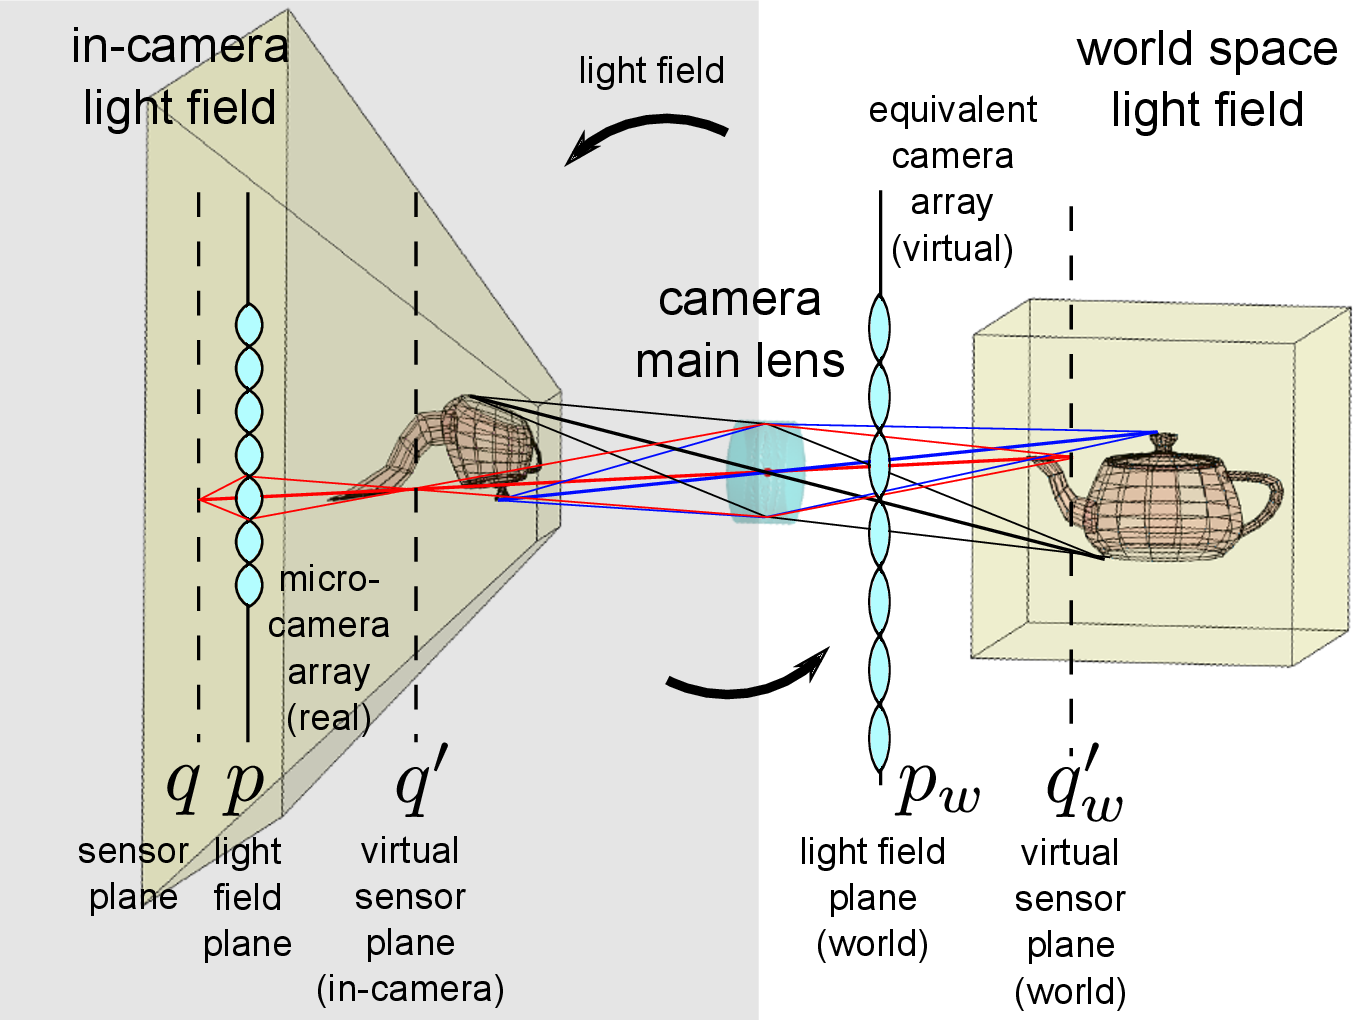
\includegraphics[width=0.9\textwidth]{images/light_field_camera.png}
    \captionof{figure}{Nguyên lý hoạt động của Camera Trường sáng. Một mảng vi thấu kính được đặt trước cảm biến. Mỗi vi thấu kính tạo ra một hình ảnh nhỏ của thấu kính chính trên các pixel bên dưới nó. Bằng cách phân tích các hình ảnh nhỏ này, thuật toán có thể suy ra cả vị trí và hướng của các tia sáng đi vào camera.}
    \label{fig:light_field_camera}
\end{center}

\subsubsection{Ứng dụng: Lấy nét lại và Thay đổi góc nhìn}
\label{subsubsec:light_field_applications}
Với trường sáng 4D, chúng ta có thể thực hiện các phép tính toán mà trước đây là không thể:
\begin{description}
    \item[Lấy nét lại Kỹ thuật số (Digital Refocusing):] Một bức ảnh truyền thống tương đương với việc tích hợp trường sáng theo một cách cụ thể để mô phỏng một mặt phẳng tiêu cự. Bằng cách thay đổi cách tích hợp này về mặt thuật toán, chúng ta có thể mô phỏng việc lấy nét ở bất kỳ độ sâu nào sau khi ảnh đã được chụp.
    \item[Thay đổi Góc nhìn (Varying Viewpoint):] Bằng cách trích xuất các lát cắt khác nhau của trường sáng 4D, chúng ta có thể tạo ra các hình ảnh của cảnh từ các góc nhìn hơi khác nhau, tạo ra hiệu ứng thị sai (parallax) nhỏ. Điều này rất hữu ích cho việc ước lượng chiều sâu (depth estimation) và tái tạo 3D.
\end{description}
Sự đánh đổi chính của ảnh trường sáng là sự đánh đổi giữa độ phân giải không gian và độ phân giải góc. Với cùng một cảm biến, ảnh trường sáng sẽ có độ phân giải không gian thấp hơn ảnh truyền thống, vì các pixel được dùng để mã hóa thông tin hướng thay vì chỉ thông tin không gian.

\section*{Tài liệu tham khảo}
\begin{itemize}
    \item[1] Gallego, G. et al. Event-based Vision: A Survey. \textit{IEEE Transactions on Pattern Analysis and Machine Intelligence} \textbf{2020}, \textit{44}(1), 154-180. (Bài tổng quan toàn diện và kinh điển về thị giác dựa trên sự kiện).
    \item[2] Chakravarthi, B. et al. Recent Event Camera Innovations: A Survey. \textit{arXiv preprint arXiv:2408.13627} \textbf{2024}.
    \item[3] Lu, Y. et al. From Events to Enhancement: A Survey on Event-Based Imaging Technologies. \textit{arXiv preprint arXiv:2505.05488} \textbf{2025}.
    \item[4] Debevec, P. E.; Malik, J. Recovering high dynamic range radiance maps from photographs. In \textit{Proceedings of the 24th annual conference on Computer graphics and interactive techniques (SIGGRAPH '97)}, 1997. (Bài báo nền tảng khai sinh ra kỹ thuật HDR hiện đại).
    \item[5] Wang, L.; Yoon, K.-J. Deep Learning for HDR Imaging: State-of-the-Art and Future Trends. \textit{arXiv preprint arXiv:2110.10394} \textbf{2021}.
    \item[6] de Lima Martins, G. et al. A Review Toward Deep Learning for High Dynamic Range Reconstruction. \textit{Applied Sciences} \textbf{2025}, \textit{15}, 5339.
    \item[7] Adelson, E. H.; Bergen, J. R. The plenoptic function and the elements of early vision. In \textit{Computational models of visual processing}, 1991. (Bài báo giới thiệu khái niệm hàm Plenoptic).
    \item[8] Ng, R. et al. Light field photography with a hand-held plenoptic camera. \textit{Stanford University Computer Science Technical Report CSTR 2005-02}, 2005. (Bài báo kinh điển về camera trường sáng cầm tay).
    \item[9] Wang, T. et al. Light field depth estimation: A comprehensive survey of principles to future. \textit{High-Confidence Computing} \textbf{2024}, \textit{4}, 100187.
    \item[10] Shannon, C. E. A Mathematical Theory of Communication. \textit{The Bell System Technical Journal} \textbf{1948}, \textit{27}(3), 379-423.
\end{itemize}